\documentclass[portrait]{poster}

\usepackage{minted}
\begin{document}

\printheader

\begin{center}
    %% TITLE
    \textbf{\bf\veryHuge\color{NavyBlue}Practical usage of Zero-knowledge in different use-cases in blockchains\\[1.5cm]}

    %% AUTHORS
    \huge     Lukáš Častven \\[0.2cm]
    \Large    \texttt{xcastven@stuba.sk}
\end{center}

\vspace{2cm}

\Large

\begin{multicols}{2}

\section*{Introduction}

    Zero Knowledge Proofs (ZKPs) provide a unique way to prove information without
    actually revealing the information itself\cite{Goldwasser1989, goldreich1991proofs}.
    This makes them ideal for
    enhancing anonymity and privacy in blockchain networks. This work
    explores the use of ZKPs to create stealth addresses on Ethereum blockchain
    \cite{ButerinIncompleteGuide}.

    ZKPs replace elliptic curve cryptography in stealth address schemas.
    This provides another method for proving ownership of a stealth
    address while protecting the recipient's identity.

\section*{Contributions}

    \begin{enumerate}
        \item \textbf{Blockchain Privacy Advancement:} This work highlights the power
            of ZKPs in developing privacy-focused cryptocurrency solutions.
        \item \textbf{ZKPs for Stealth Addresses:} Successful demonstration of using
            ZKPs in designing stealth address schema.
        \item \textbf{Trustless Ownership Proof: } Proposed scheme enables trustless
            proof of stealth address ownership without compromising privacy.
    \end{enumerate}

\section*{Solution Design}

    The core principle behind the solution is that both receiver
    and sender generate a random value\cite{ButerinIncompleteGuide}.
    These two values can then
    be used to prove to a stealth address that whoever owns these
    values is the owner of the stealth address, and can control it.

    Bob, as a receiver, publishes the hash of his random value to a public
    registry. With this hash he also publishes his public key, which corresponds
    to his private key. This tuple is Bob's meta stealth address, visualized in Figure
    \ref{fig:bobs-meta-address}.

    \begin{center}\vspace{1cm}
        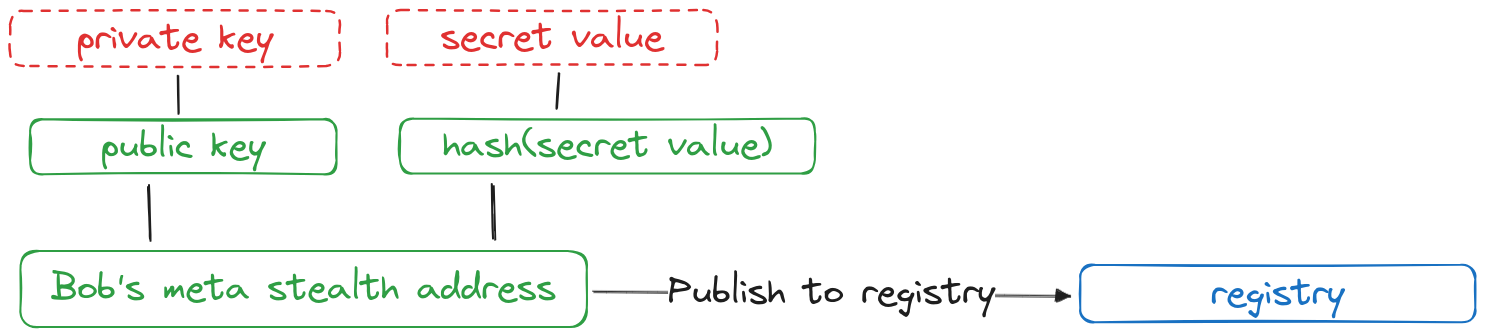
\includegraphics[width=0.7\linewidth]{./assets/meta-stealth-address.png}
        \captionof{figure}{Bob's Meta Stealth Address}
        \label{fig:bobs-meta-address}
    \end{center}\vspace{1cm}

    When Alice wants to send funds to Bob, she finds his meta stealth address
    in the public registry, generates her own random value and hashes it together
    with Bob's hash to create a code. Then she deploys a new stealth wallet
    contract with this code in it, and amount of funds that she wanted to send
    to Bob. After that, she encrypts her random value with Bob's public key,
    this encrypted value is called ephemeral key. Alice publishes it to a
    public registry. This whole process is depicted in Figure \ref{fig:sending-funds}. 

    \begin{center}\vspace{1cm}
        \centering
        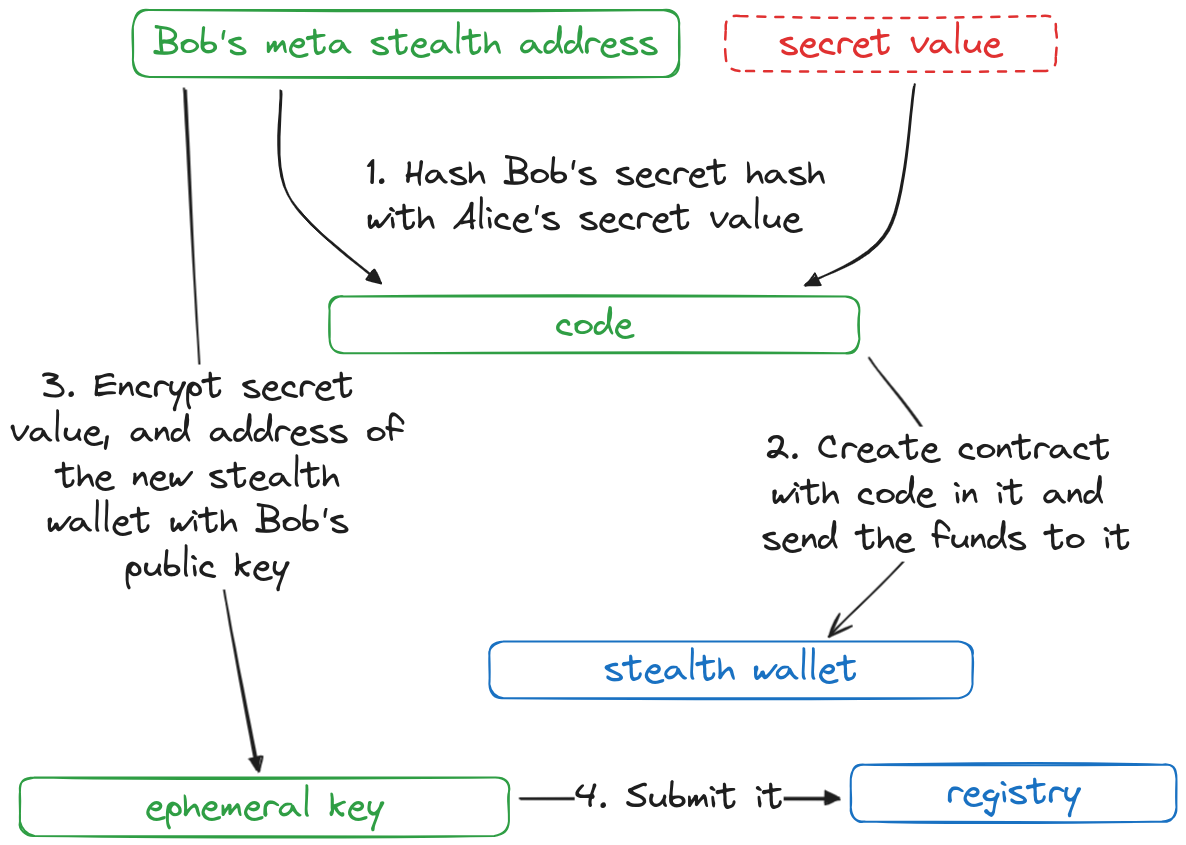
\includegraphics[width=0.5\linewidth]{../iitsrc/assets/images/sending-funds.png}
        \captionof{figure}{Alice sends funds}
        \label{fig:sending-funds}
    \end{center}\vspace{1cm}

    Bob then scans the registry, tries to decrypt ephemeral keys. When the
    decryption is successful, Bob can save the decrypted Alice's secret value
    and the address of the corresponding stealth wallet.

    \begin{center}\vspace{1cm}
        \centering
        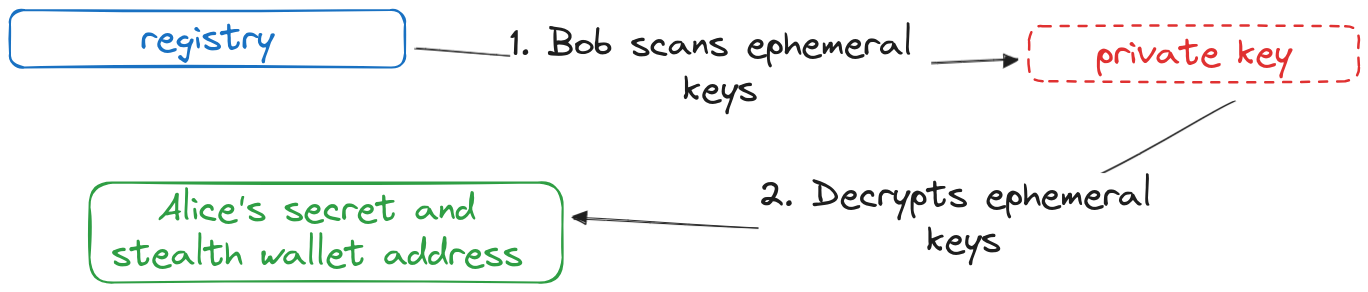
\includegraphics[width=0.7\linewidth]{./assets/scanning-ephemeral-keys.png}
        \captionof{figure}{Bob scans ephemeral keys}
        \label{fig:scanning-ephemeral-keys}
    \end{center}\vspace{1cm}


    To use the funds, Bob must generate a ZK proof and submit it to the stealth
    wallet. This proof proves that Bob knows Alice's random value
    and his own random value, such that
    \[ code = hash(hash(Bob's\:value),\:Alice's\:value) \]
    where $code$ is the one submitted by Alice into the stealth wallet contract.

    \begin{center}\vspace{1cm}
        \centering
        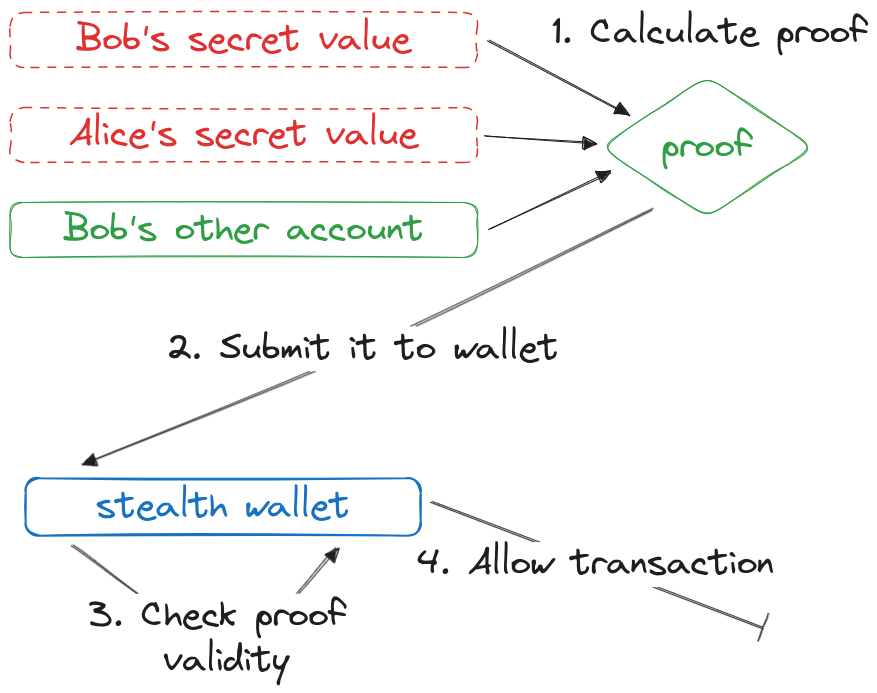
\includegraphics[width=0.4\linewidth]{../iitsrc/assets/images/interating-with-wallet.png}
        \captionof{figure}{Bob's interaction with wallet}
        \label{fig:wallet-interaction}
    \end{center}\vspace{1cm}

    The proof is computed and validated according to this Circom circuit:

    \begin{center}\vspace{1cm}
        \centering
        \begin{minted}[fontsize=\small]{c}
            pragma circom 2.0.0;
            include "./circomlib/circuits/poseidon.circom";

            template Ownership() {
                signal input owner_secret;
                signal input sender_secret;
                signal input code;
                signal input withdrawee_address;
                signal input msg_sender;

                component owner_secret_poseidon = Poseidon(1);
                owner_secret_poseidon.inputs <== [owner_secret];

                component code_poseidon = Poseidon(2);
                code_poseidon.inputs <== [owner_secret_poseidon.out, sender_secret];

                code === code_poseidon.out;
                msg_sender === withdrawee_address;
            }
            component main {public [code, msg_sender]} = Ownership();
        \end{minted}
        \captionof{figure}{Circom circuit for proving ownership}
        \label{fig:circuit}
    \end{center}\vspace{1cm}

\section*{Conclusions}

    This work demonstrates a successful use of Zero-Knowledge Proofs
    to enhance privacy on Ethereum blockchain. By
    utilizing ZKPs to prove stealth address ownership, it offers a novel
    approach to protect transaction participants identities. This work
    highlights the potential of ZKPs to significantly improve
    blockchain anonymity.


\bibliographystyle{plain}
\bibliography{refs}

\end{multicols}
\end{document}
